\documentclass{oblivoir}
\usepackage{amsmath,amssymb,amsthm,kotex,mdframed,paralist,tabto,pifont}

\counterwithout{subsection}{section}
\newcounter{num}
\newcommand{\prob}[1]
{\bigskip\noindent\refstepcounter{num}\subsection{#1}}

\newcommand{\ans}{
{\par\medskip\begin{mdframed}
\textbf{풀이 : }
\vspace{0.6\textheight}
\end{mdframed}\par
\raggedleft\textbf{답 : (\qquad\qquad\qquad\qquad\qquad\qquad)}
\par}\bigskip\bigskip}

\newcommand\ov[2]{\ensuremath{\overline{#1#2}}}

\newcommand\ve[2]{\ensuremath{\overrightarrow{#1#2}}}

\newcommand{\pa}{\mathbin{\!/\mkern-5mu/\!}}

\TabPositions{0.2\textwidth,0.4\textwidth,0.6\textwidth,0.8\textwidth}
\newcommand\tabb[5]{\par\noindent
\ding{172}{#1}
\tab\ding{173}{#2}
\tab\ding{174}{#3}
\tab\ding{175}{#4}
\tab\ding{176}{#5}}

\newcounter{pnum}
\newcommand\pn{\stepcounter{pnum}\textbf{\thepnum}}

%%%
\begin{document}
\title{혜령 10 - 기하와 벡터[수능특강]\\
{\large 9단원 : 도형의 방정식}}
\author{}
\date{\today}
\maketitle
\tableofcontents

\newpage

%
\prob{09-예제2}
좌표공간의 점 \(A\)에서 만나는 두 직선 \(l:-x+3=\frac y5=z-2\), \(m:x-2=y+1=-z+3\)이 있다.
직선 \(l\)위의 점 \(P\)에서 직선 \(m\)에 내린 수선의 발을 \(H\)라고 할 때, \(\ov PH=4\)이다.
선분 \(AP\)의 길이는?
\tabb{\(\sqrt{15}\)}{\(4\)}{\(\sqrt{17}\)}{\(3\sqrt2\)}{\(\sqrt{19}\)}

%
\prob{09-유제3}
좌표공간에서 직선 \(\frac{x-3}2=\frac{y+1}a=-z\)가 직선 \(-x=-\frac12y+3=bz+1\)에 평행하고 직선 \(\frac{x+2}2=\frac{-y+3}2=\frac zc\)와 수직일 때, 세 상수 \(a\), \(b\), \(c\)에 대하여 \(a+b+c\)의 값은?
(단, \(abc\neq0\))
\tabb01234

%
\prob{09-유제4}
좌표공간의 점 \(A(1,3,-2)\)에서 직선 \(x=\frac{y-5}2=\frac{z-10}2\)에 내린 수선의 발을 \(H(a,b,c)\)라고 할 때, \(a+b+c\)의 값은?
\tabb01234

%
\prob{09-예제3}
좌표공간에서 점 \(A(2,-3,1)\)를 지나고 두 평면 \(x+y+z=5\), \(2x+y+z=6\)에 각각 수직인 평면을 \(\alpha\)라고 하자.
점 \(P=(3,0,k)\)가 평면 \(\alpha\) 위의 점일 때, \(k\)의 값은?
\tabb01234
\newpage

%
\prob{09-예제4}
좌표 공간의 두 점 \(A=(1,5,-4)\), \(B(3,1,2)\)와 임의의 점 \(P\)의 위치벡터를 각각 \(\vec a\), \(\vec b\), \(\vec x\)라고 할 때, 다음 조건을 만족시키는 점 \(P\)가 나타내는 도형을 \(S\)라고 하자.
\[(\vec x-\vec a)\textbullet(\vec x-\vec b)=\vec0\]
도형 \(S\)와 평면 \(x-z+1=0\)이 만나서 생기는 도형의 넓이는?
\tabb{\(6\pi\)}{\(8\pi\)}{\(10\pi\)}{\(12\pi\)}{\(14\pi\)}

%
\prob{09-유제8}
좌표공간의 두 점 \(A(3,-4,1)\), \(B(1,0,3)\)에 대하여 \(\ve AP\textbullet\ve BP=0\)을 만족시키는 점 \(P\)가 나타내는 도형을 \(T\)라고 하고, 원점 \(O\)를 지나는 직선이 도형 \(T\)와 한 점에서만 만날 때 그 점을 \(Q\)라고 하자.
선분 \(OQ\)의 길이를 \(l\)이라고 할 때, \(l^2\)의 값을 구하시오.
\tabb{\(3\)}{\(6\)}{\(9\)}{\(12\)}{\(15\)}

%
\prob{09-기초3}
좌표공간에서 매개변수 \(t\)로 나타낸 직선 \(x=3t-1\), \(y=t\), \(z=\frac12t+5\) (\(t\)는 실수)에 수직이고 점 \((3,-1,2)\)를 지나는 평면의 방정식은 \(6x+ay+bz+c=0\)이다.
세 상수 \(a\), \(b\), \(c\)에 대하여 \(a+b+c\)의 값을 구하시오.
\tabb{\(-18\)}{\(-15\)}{\(-12\)}{\(-9\)}{\(-6\)}

%
\prob{09-기초3-1}
좌표공간에서 점 \(A(3,-2,-1)\)와 법선벡터가 \((4,-4,7)\)인 평면 \(\alpha\) 사이의 거리가 \(3\)일 때, 평면 \(\alpha\)는 \(z\)축과 점 \(P(0,0,-k)\)에서 만난다.
양수 \(k\)의 값을 구하시오.
\tabb{\(2\)}{\(6\)}{\(10\)}{\(14\)}{\(18\)}
\newpage

%
\prob{09-기초3-2}
좌표공간에서 점 \(A(2,5,0)\)의 위치벡터를 \(\vec a\)라고 하자.
벡터 \(\vec u=(1,-1,2)\)에 대해 \(\vec p=\vec a+t\vec u\)(\(t\)는 실수)를 만족시키는 점 \(P\)가 나타내는 직선과 \(x\)축이 이루는 각도를 \(\theta\)라고 할 때 \(\cos^2\theta\)의 값을 구하여라.
(단, \(\vec p\)는 점 \(P\)의 위치벡터이다.)
\tabb{\(\frac12\)}{\(\frac13\)}{\(\frac14\)}{\(\frac15\)}{\(\frac16\)}

%
\prob{09-기본1}
좌표공간에서 직선 \(\frac{x-3}2=\frac{y-3}3=-\frac z6\)의 \(y\ge0\), \(z\ge0\)인 부분의 길이는?
\tabb{\(3\sqrt5\)}{\(\sqrt{46}\)}{\(\sqrt{47}\)}{\(4\sqrt3\)}{\(7\)}

%
\prob{09-기본2}
좌표공간에서 점 \(A(1,1,0)\)을 지나는 직선 \(l\)이 다음 조건을 만족시킨다.
\begin{enumerate}\tightlist
\item[(가)]
직선 \(l\)의 \(xy\)평면 위로의 정사영의 방정식은 \(x+y=2\), \(z=0\)이다.
\item[(나)]
직선 \(l\)과 \(z\)축이 이루는 예각의 크기는 \(\frac\pi6\)이다.
\end{enumerate}
직선 \(l\)이 \(yz\)평면과 만나는 점을 \(P\)라고 할 때, 삼각형 \(OAP\)의 넓이는?
(단 \(O\)는 원점이고, \(P\)의 \(z\)좌표는 양수이다.)
\tabb{\(1\)}{\(\sqrt2\)}{\(\sqrt3\)}{\(2\)}{\(5\)}

%
\prob{09-기본3}
좌표공간에 점 \(A(1,-3,5)\)과 임의의 점 \(P\)가 있다. \(\ve OA=\vec a\), \(\ve OP=\vec x\)라고 할 때, 방정식 \((\vec x-\vec a)\textbullet(\vec x-\vec a)=6\)을 만족시키는 점 \(P\)와 직선 \(x-6=\frac{y-8}4=-\frac{z+2}2\) 사이의 거리의 최댓값은?
(단, \(O\)는 원점이다.)
\tabb{\(\sqrt6\)}{\(2\sqrt6\)}{\(3\sqrt6\)}{\(4\sqrt6\)}{\(5\sqrt6\)}
\newpage

%
\prob{09-기본5}
좌표공간의 두 점 \(A(4,-3,-5)\), \(B(3,5,-1)\)에서 같은 거리에 있는 점 \(P\)가 나타내는 도형이 평면 \(x=3\)와 이루는 각의 크기를 \(\theta(0\le\theta\le\frac\pi2)\)라고 할 때, \(\cos\theta\)의 값은?
\tabb{\(\frac19\)}{\(\frac29\)}{\(\frac13\)}{\(\frac49\)}{\(\frac59\)}

%
\prob{09-기본6}
좌표공간에서 두 직선 \(\frac{x-1}3=-y=z+5\), \(\frac{x+5}2=y-3=\frac z4\)을 포함하는 평면을 \(\alpha\)라고 하자.
\(y\)축과 평면 \(\alpha\)가 이루는 각의 크기를 \(\theta(0\le\theta\le\frac\pi2)\)라고 할 때, \(\sin\theta\)의 값은?
\tabb{\(\frac{\sqrt3}3\)}{\(\frac23\)}{\(\frac{\sqrt5}3\)}{\(\frac{\sqrt6}3\)}{\(\frac{\sqrt7}3\)}

%
\prob{09-기본7}
좌표공간에서 높이가 \(3\)인 원기둥의 두 밑면이 각각 평면 \(2x-6y+3z=0\), \(ax+by+cz+21=0\) 위에 놓여 있다.
세 상수 \(a\), \(b\), \(c\)에 대하여 \(a^2+b^2+c^2\)의 값을 구하시오.
\tabb{\(16\)}{\(25\)}{\(36\)}{\(49\)}{\(64\)}
\newpage

%
\prob{09-기본8}
좌표공간에서 평면 \(x+y+z=1\)이 \(x\)축, \(y\)축, \(z\)축과 만나는 점을 각각 \(A\), \(B\), \(C\)라고 할 때, 평면 \(y=5\) 위의 점 \(P(a,5,b)\)에 대하여 사면체 \(PABC\)는 다음 조건을 만족시킨다.
\begin{enumerate}
\item[(가)]
두 삼각형 \(PCA\)와 \(PCB\)의 넓이가 서로 같다.
\item[(나)]
사면체 \(PABC\)의 부피는 \(9\)이다.
\end{enumerate}
\(\frac ba\)의 최댓값은?
\begin{figure}[h!]
\centering
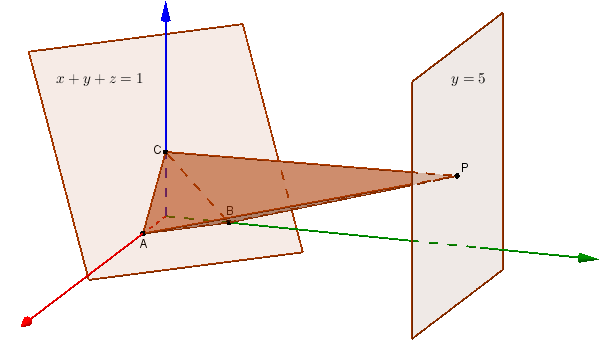
\includegraphics[width=0.9\textwidth]{01}
\end{figure}
\tabb6789{10}
\newpage

%
\prob{09-실력1}
그림과 같이 두 밑면 \(ABCD\), \(EFGH\)는 한 변의 길이가 \(\sqrt2\)인 마름모이고 네 옆면은 정사각형인 육면체 \(ABCD-EFGH\)를 세 점 \(E\), \(F\), \(H\)의 좌표가 각각 \(E(0,0,1)\), \(F(1,0,0)\), \(H(0,1,0)\)이 되도록 좌표공간에 놓았다.
두 점 \(BC\)를 지나는 직선이 \(xy\)평면과 만나는 점을 \(P(a,b,0)\)이라고 할 때, \(a+b\)의 값은?
(단, 점 \(A\)의 좌표는 양수이다.)
\begin{figure}[h!]
\centering
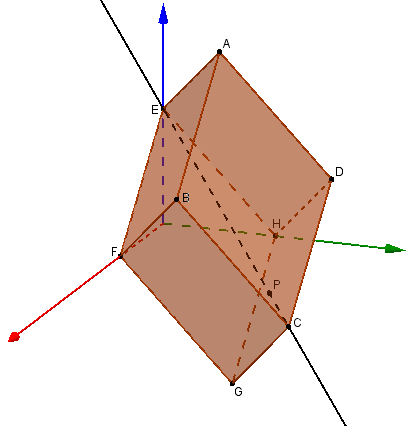
\includegraphics[width=0.5\textwidth]{02}
\end{figure}
\tabb{\(\frac{8+\sqrt6}5\)}{\(\frac{8+2\sqrt6}5\)}{\(\frac{8+3\sqrt6}5\)}{\(\frac{4+\sqrt6}5\)}{\(\frac{4+2\sqrt6}5\)}

%
\prob{09-실력2}
좌표평면에서 \(xy\)평면, \(yz\)평면, \(zx\)평면에 동시에 접하면서 반지름의 길이가 \(1\)인 구를 \(S_1\)이라고 하고, \(xy\)평면, \(yz\)평면, 구 \(S_1\)에 동시에 접하면서 반지름의 길이가 \(2\)인 구를 \(S_2\)라고 하자.
두 구 \(S_1\), \(S_2\)의 중심을 각각 \(A\), \(B\)라 하고 점 \(C\)의 좌표가 \((0,0,2)\)일 때, 삼각형 \(ABC\)의 넓이는?
(단, 두 점 \(A\), \(B\)의 \(x\)좌표, \(y\)좌표, \(z\)좌표는 모두 양수이다.)
\tabb{\(1\)}{\(\sqrt2\)}{\(\sqrt3\)}{\(2\)}{\(\sqrt5\)}
\newpage

%
\prob{09-실력3}
그림과 같이 모든 모서리의 길이가 \(2\)인 사각뿔 \(A-BCDE\)에서 삼각형 \(ACD\)의 무게중심을 \(G\)라고 하자.
점 \(P\)가 선분 \(BG\)위의 점일 때, \(\ve PB\textbullet\ve PD\)의 최솟값은?
\begin{figure}[h!]
\centering
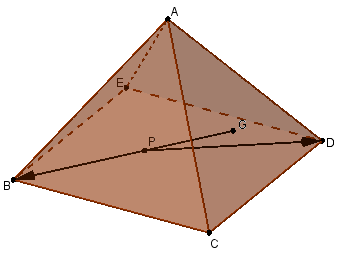
\includegraphics[width=0.5\textwidth]{03}
\end{figure}
\tabb{\(-\frac19\)}{\(-\frac49\)}{\(-1\)}{\(-\frac{16}9\)}{\(-\frac{25}9\)}
\newpage

%
\prob{09-실력5}
그림과 같이 \(\ov AB=1\), \(\ov AD=2\), \(\ov AE=1\)인 직육면체 \(ABCD-EFGH\)를 세 점 \(A\), \(F\), \(H\)의 좌표가 각각 \(A(0,0,1)\), \(F(1,0,0)\), \(H(0,2,0)\)이 되도록 좌표공간에 놓았다.
\\
두 선분 \(AD\), \(BC\)를 3:1로 내분하는 점을 각각 \(I\), \(J\)라고 하고 두 선분 \(FG\), \(EH\)의 중점을 각각 \(K\), \(L\)이라고 하자.
직선 \(AG\)와 평면 \(IJKL\)이 만나는 점을 \(P\)라고 할 때, 직선 \(DP\)와 \(xy\)평면이 만나는 점의 좌표를 \((a,b,c)\)라고 하자.
\(a+b+c\)의 값은?
\begin{figure}[h!]
\centering
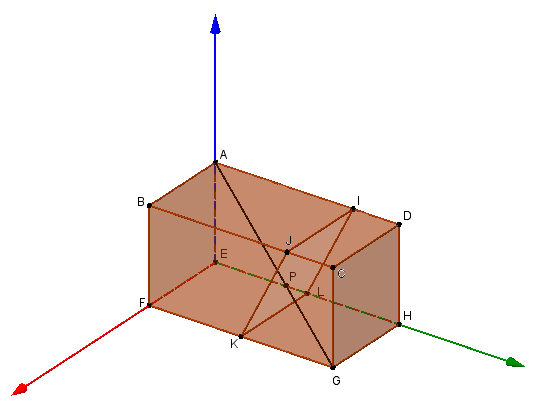
\includegraphics[width=0.7\textwidth]{04}
\end{figure}
\tabb{\(\frac13\)}{\(\frac23\)}{\(1\)}{\(\frac43\)}{\(\frac53\)}

%
\prob{09-기출}
좌표공간에서 직선 \(l:x=\frac{y-2}3=\frac{3-z}2\)와 평면 \(\alpha\)가 점 \(P(2,8,-1)\)에서 수직으로 만난다.
직선 \(l\) 위의 점 \(A(a,b,c)\)와 평면 \(\alpha\) 위의 점 \(Q\)에 대하여 \(\ve AP\textbullet\ve AQ=14\)일 때 \(a+b+c\)의 값은?
(단, \(c>0\))
\tabb34567
\newpage

%%%%
\begin{table}[h!]
\begin{tabular}{|c|c||c|c||c|c||c|c|}
\hline
\pn&\ding{175}	&\pn&\ding{174}	&\pn&\ding{172}	&\pn&\ding{176}\\\hline
\pn&\ding{172}	&\pn&\ding{173}	&\pn&\ding{173}	&\pn&\ding{172}\\\hline
\pn&\ding{176}	&\pn&\ding{176}	&\pn&\ding{175}	&\pn&\ding{173}\\\hline
\pn&\ding{172}	&\pn&\ding{175}	&\pn&\ding{175}	&\pn&\ding{175}\\\hline
\pn&\ding{174}	&\pn&\ding{176}	&\pn&\ding{175}	&\pn&\ding{176}\\\hline
\pn&\ding{176}	&&&&&&\\\hline
\end{tabular}
\end{table}
\end{document}